\documentclass[10pt]{beamer}
\usepackage{tikz} % affichage de schémas
\usepackage{float} % placement des figures
\usepackage{amssymb} % symboles mathématiques
\usepackage[T1]{fontenc} % encodage
\usepackage[french]{babel} % gestion du français
\usepackage{verbatim}
\usepackage{color}
\usepackage[utf8]{inputenc} % encodage

\usepackage{textcomp} % flèche,  intervalle
\usepackage{stmaryrd} % intervalle entiers

\usepackage{amsthm} % format des déf, prop...
\usepackage{amsmath} % matrices, ...
\usepackage{multirow} % fusionner cellules verticalement

\usepackage{graphicx} % affichage d'images
\usepackage{bbold} % fonction caractéristique 1
\usepackage{xcolor} % couleur dans math

\definecolor{bgreen}{rgb}{0.30,0.70,0}

%#############################################################################################################%
%#############################################################################################################%
%#############################################################################################################%

\usetheme{Amsterdam}

\setbeamertemplate{footline}%{miniframes theme}
  {
    \begin{beamercolorbox}[ht=2.5ex,dp=1.125ex,%
      leftskip=.3cm,rightskip=.3cm plus1fil]{title in head/foot}%
      {\usebeamerfont{title in head/foot}\insertshorttitle} - Yassine Hamoudi  \hfill   \insertframenumber/\inserttotalframenumber
    \end{beamercolorbox}%
  }

%#############################################################################################################%
%#############################################################################################################%
%#############################################################################################################%

\title{Literature review  \\ Natural Language Question Answering}
\author{{\Large Yassine \textsc{Hamoudi}}}
\date{October 7, 2014}

\begin{document}

%#############################################################################################################%

\begin{frame}
  \titlepage
\end{frame}

%#############################################################################################################%

\begin{frame}{Introduction}

\begin{alertblock}{Problematic}
 How answering natural language questions using existing structured databases?
\end{alertblock}

\onslide<2->{
Objectives:
\begin{itemize}
	\item question processing module: transform questions into normal form.
	\item databases processing module: find answers in databases.
	\item answer extraction module: return the exact answers, extracted after the previous step.	
\end{itemize}
}

\end{frame}

%#############################################################################################################%

\begin{frame}

What we want to do:
	\begin{itemize}
		\item strong normalization of questions.
		\item searching answers in highly structured databases.
		\item full modular tool, to plug in easily as many databases as possible.
	\end{itemize}

\onslide<2->{
What we do not plan to do (?):
	\begin{itemize}
		\item searching answers in not structured corpus of texts (newspapers, books...).
		\item trying to directly find sentences that best match with the question and probably contain the answer.
	\end{itemize}
}

\onslide<3->{	
\begin{alertblock}{Warning}
	Most of the existing papers deal with the second kind of question answering. Their techniques cannot be directly applied to our subject.
\end{alertblock}
}

\end{frame}

%#############################################################################################################%

\begin{frame}{Normal form representation}

\section{Normal form representation}

Most common representation: Subject Predicate Object (SPO)

\begin{exampleblock}{Example}
		The turtle eats a salad. 
		\begin{center}
		SPO = (turtle,eats,salad) or eats(turtle,salad)
		\end{center}
\end{exampleblock}

\onslide<2->{
Expressing questions in first order logic:
\begin{itemize}
	\item What is the birth date of the first president of the USA?
		\begin{itemize}
			\item[$\rightarrow$] $\exists x \exists y$, be(x,first president of the USA) $\wedge$ wasBornIn(x,y)
		\end{itemize}
	\onslide<3->{
	\item What is the capital of the southest African state?
		\begin{itemize}
			\item[$\rightarrow$] $\exists x \exists y$, southestOf(x,Africa) $\wedge$ isCapitalOf(y,x)
		\end{itemize}
	}
	\onslide<4->{
	\item What is the name of the actress that played in Pocahontas and is married to a French violonist?
		\begin{itemize}
			\item[$\rightarrow$] $\exists x \exists y$, hasGender(x,woman) $\wedge$ playedIn(x,Pocahontas) $\wedge$ isMarriedTo(x,y) $\wedge$ hasNationality(y,French) $\wedge$ hasJob(y,violonist)
	}
		\end{itemize}
\end{itemize}			
}

\end{frame}

%#############################################################################################################%

\begin{frame}

	\begin{center}
		Finding the answer $\Leftrightarrow$ finding a model in first order logic
	\end{center}
	
	\begin{itemize}
		\item Each triplet conducts to quering a database:
				\begin{itemize}
					\item[$\rightarrow$] playedIn(x,Pocahontas) $\hookrightarrow$ IMBd
					\item[$\rightarrow$] hasJob(y,violonist) $\hookrightarrow$ MusicBrainz
					\item[$\rightarrow$] $\dots$
				\end{itemize}
		\item Combining the answer to get the final result.
		\item More complex model: allowing universal quantification, negation...
	\end{itemize}

\end{frame}

%#############################################################################################################%

\begin{frame}

\begin{exampleblock}{RDF (Resource Description Framework)}
	\begin{itemize}
		\item general framework for describing any Internet resource.
		\item a RDF document is a set of triplets (subject,predicate,object).
		\item \url{http://fr.wikipedia.org/wiki/Resource_Description_Framework}
		\item \url{http://www.w3.org/2001/sw/SW-FAQ\#whrdf}
	\end{itemize}
\end{exampleblock}

\onslide<2->{
\begin{exampleblock}{SPARQL (SPARQL Protocol and RDF Query Language)}
	\begin{itemize}
		\item an RDF query language.
		\item a W3C recommendation, fully standardized.
		\item can be used with a lot of knowledge bases.
	\end{itemize} 
\end{exampleblock}
}
		
\end{frame}

%#############################################################################################################%

\begin{frame}

Existing knowledge bases

\begin{itemize}
	\item YAGO2: more than 10 million entities and more than 120 million facts about these entities.
	\item DBpedia: 4.58 million entities, out of which 4.22 are classified in a consistent ontology.
	\item Freebase
	\item MusicBrainz
	\item \textbf{Wikidata}
	\item IMDb (Internet Movie Database)
	\item ...
\end{itemize}

\begin{itemize}
	\item[$\rightarrow$] most of them can be accessed via SPARQL queries (Wikidata?).
	\item[$\rightarrow$] more than 100 public SPARQL endpoints with dozens of billion of triples (\url{http://www.w3.org/wiki/SparqlEndpoints} for some examples).
	\item[$\rightarrow$] more and more SPARQL endpoints in the future.
\end{itemize}

\end{frame}

%#############################################################################################################%

\begin{frame}
 
\begin{alertblock}{Changing our goals (?):}
	\begin{itemize}
		\item using SPARQL language (even if it is not the best tool to deal with wikidata?).
		\item restricted modularity: only able to plug-in via SPARQL endpoint.
		\item designing a tool that deals with the wide range of SPARQL endpoints.
	\end{itemize}
\end{alertblock}

\end{frame}

%#############################################################################################################%

\begin{frame}{From syntax...}

\section{From syntax...}

\begin{block}{Parse structure tree (constituency relations)}
	Split the phrase according to its grammatical structure (noun phrase: NP, verb phrase: VP ...).
	\begin{center}
		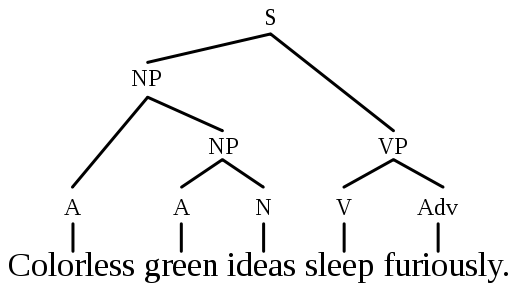
\includegraphics[scale=0.30]{522px-Cgisf-tgg.png}
	\end{center}
\end{block}
		
\end{frame}

%#############################################################################################################%

\begin{frame}

\begin{block}{Dependency tree (dependency relations)}
	Reflect grammatical relationships between words in a sentence.
	\begin{center}
		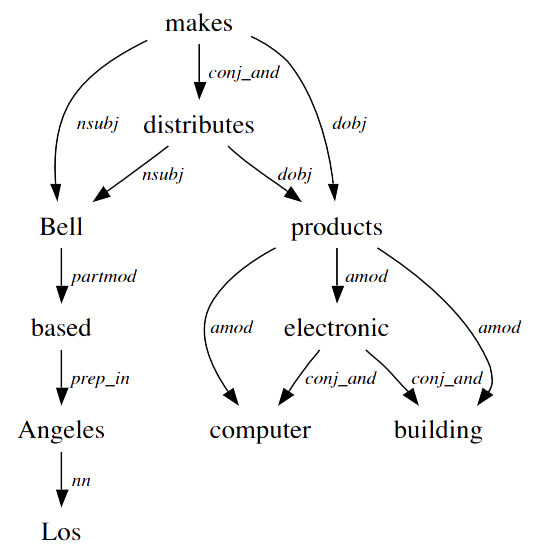
\includegraphics[scale=0.40]{depen.png}
			
		\textit{Bell, based in Los Angeles, makes and distributes electronic, computer and building products.}
	\end{center}
\end{block}

Stanford Parser:
	- provides a state-of-the-art dependency parser.
	- Stanford typed dependencies manual : \url{http://nlp.stanford.edu/software/dependencies_manual.pdf}.
		
\end{frame}

%#############################################################################################################%

\begin{frame}{... to semantic}

\section{... to semantic}

Parse structure tree 
\begin{itemize}
	\item not the best way to deal with semantic.
	\item an algorithm : \url{http://ailab.ijs.si/delia_rusu/Papers/is_2007.pdf}. Not very effective...
\end{itemize}

\onslide<2->{
Dependency tree
\begin{itemize}
	\item commonly used to perform triplet extraction.
	\item no good articles found on how to perform this.
\end{itemize}
}

\onslide<3->{
Other approachs: 
\begin{itemize}
	\item machine learning
	\item linear programming
	\item ...
\end{itemize}

$\rightarrow$ usually a mix of heuristics (including parse structure/dependency tree)
}
		
\end{frame}

%#############################################################################################################%

\begin{frame}{Libraries}

\section{Libraries}

\begin{exampleblock}{NLTK: \url{http://www.nltk.org/}}
	\begin{itemize}
		\item[+] python
		\item[+] well documented, easy to use
		\item[-] slow (according to many users)
		\item[-] \textcolor{red}{no statistical parser.} Concretely : we cannot use it as is. Extra libraries : 
				\begin{itemize}
					\item \url{http://stackoverflow.com/questions/6115677/english-grammar-for-parsing-in-nltk}
					\item \url{http://stackoverflow.com/questions/14009330/how-to-use-malt-parser-in-python-nltk}
				\end{itemize}
	\end{itemize}
\end{exampleblock}

\end{frame}

%#############################################################################################################%

\begin{frame}

\begin{exampleblock}{Stanford Parser: \url{http://nlp.stanford.edu/}}
	\begin{itemize}
		\item[+] well documented
		\item[+] faster than NLTK
		\item[+] frequently updated. A "state of the art" tool.
		\item[+] include a (the best ?) \textcolor{red}{dependency parser}: \url{http://nlp.stanford.edu/software/dependencies_manual.pdf}
		\item[-] java?
	\end{itemize}
	
Online demo : 
	\begin{itemize}
		\item \url{http://nlp.stanford.edu:8080/parser/index.jsp}
		\item (coreNLP): \url{http://nlp.stanford.edu:8080/corenlp/process}
	\end{itemize}
\end{exampleblock}

\textbf{Other tools:} OpenNLP, Link Parser, Minipar, Berkeley Parser (online demo: \url{http://tomato.banatao.berkeley.edu:8080/parser/parser.html})...

\end{frame}

%#############################################################################################################%

\begin{frame}{Treebanks}

\section{Treebanks}

Text corpus with annotated syntactic (=structure) or semantic (=meaning) sentence structure.

\begin{exampleblock}{Finding treebanks}
	\begin{itemize}
		\item \url{http://en.wikipedia.org/wiki/Treebank} (existing tools)
		\item Question Treebank: \url{http://www.computing.dcu.ie/~jjudge/qtreebank/} or \url{http://nlp.stanford.edu/data/QuestionBank-Stanford.shtml}
	\end{itemize}
\end{exampleblock}

\end{frame}

%#############################################################################################################%

\begin{frame}

Semi-automatic / learning methods to build treebanks (?): 
	\begin{itemize}
		\item \url{http://www.hugo-zaragoza.net/academic/pdf/atserias_lrec10.pdf}
		\item \url{http://www.researchgate.net/publication/228739113_Semi-Automatic_Construction_of_a_Question_Treebank}
	\end{itemize}
	
~\\

$\rightarrow$	Mainly syntactic treebank (syntactic parse tree).

$\rightarrow$	Some semantic treebanks (the most intereressant for machine learning ?).
	
\end{frame}

%#############################################################################################################%

\begin{frame}{Existing answering systems}

\section{Existing answering systems}

Some tools:
\begin{itemize}
	\item \url{http://quepy.machinalis.com/}
	\item \url{https://www.youtube.com/watch?v=9v5nk1bzyD4}
	\item \url{http://www.ifi.uzh.ch/ddis/research/talking.html}
\end{itemize}

Many other tools but source code not available.

~\\

Question Answering over Linked Data challenge: 
\begin{itemize}
	\item[$\rightarrow$] \url{http://greententacle.techfak.uni-bielefeld.de/~cunger/qald/}
	\item[$\rightarrow$] 2013 winner: \url{https://bitbucket.org/sebferre/squall2sparql} (from Rennes)
\end{itemize}
		
\end{frame}

%#############################################################################################################%

\begin{frame}{Conclusion}

\section{Conclusion}

\begin{itemize}
	\item Lack of details about implementation in papers actually found.
	\item Most interesting papers (?):
		\begin{itemize}
			\item[-] \url{http://adapt.seiee.sjtu.edu.cn/~kangqi/qa.html} : rewiew of \textcolor{red}{4 modern methods} about question answering to databases. 
			\item[-] \url{http://people.mpi-inf.mpg.de/~myahya/papers/EMNLP2012_yahya.pdf}
			\item[-] \url{http://www.aifb.kit.edu/images/1/12/55540445.pdf}
			\item[-] more on \url{http://pad.aliens-lyon.fr/p/ppp-nlp}
		\end{itemize}
	\item	Be aware of the difficulty of our task : very recent papers on question answering from knowledge bases claim no more than 30-50\% of success.
	\item Relaxed problems:
		\begin{itemize}
			\item[-] interactions between the system and the user to find the answer.
			\item[-] restricted grammar for asking questions (not fully "natural question answering").
		\end{itemize}
\end{itemize}


\end{frame}

%#############################################################################################################%

\begin{frame}{Keywords}

\section{Keywords}

\begin{table}
\Large
\centering
\begin{tabular}{ccc}
	\textcolor{brown}{question answering} & SPARQL & \textcolor{green}{RDF} \\
	\multicolumn{3}{c}{natural language question answering} \\ 
	\textcolor{red}{semantic parser} & \multicolumn{2}{c}{\textcolor{purple}{subject verb object}} \\
	\multicolumn{3}{c}{predicate object subject} \\
	triple(t) extraction & \multicolumn{2}{c}{\textcolor{orange}{natural language RDF/SPARQL}} \\
	\multicolumn{3}{c}{natural language interfaces to databases} \\
	\multicolumn{3}{c}{\textcolor{blue}{SVO (subject verb object)}} \\
	\multicolumn{3}{c}{\textcolor{gray}{translating questions into queries over knowledge base}}
\end{tabular}
\end{table}

\end{frame}

%#############################################################################################################%

\end{document}
